\documentclass[journal]{IEEEtran}
\usepackage{subcaption}
% --- Preamble ---
\usepackage[utf8]{inputenc}
\usepackage[T1]{fontenc}
\usepackage{amsmath, amssymb, amsfonts, amsthm}
\usepackage{graphicx}
\usepackage{cite}
\usepackage{bm}
\usepackage{algorithm}
\usepackage{algorithmic}
\usepackage{booktabs}
\usepackage{xcolor}
\usepackage{tikz}
\usepackage{pgfplots}
\usetikzlibrary{shapes, arrows, positioning, calc}
\pgfplotsset{compat=1.18}

% --- Custom Math Commands ---
\newcommand{\herm}{^{\mathsf{H}}}
\newcommand{\trans}{^{\mathsf{T}}}

\begin{document}

\title{Structural Inductive Biases in Neural Optimization: Comparative Unfolding Paradigms for Multi-IRS IoT Networks}

\author{Vesal Hakami, \IEEEmembership{Member IEEE}\\
Payam Kouchakzade}

\maketitle

\begin{abstract}
Intelligent Reflecting Surfaces (IRSs) offer massive spectral efficiency gains for 6G Internet of Things (IoT) networks, but they introduce prohibitive computational complexity for real-time resource orchestration. Classical fractional programming (FP) algorithms for Weighted Sum-Rate (WSR) maximization suffer from a severe $\mathcal{O}(M^3)$ matrix inversion bottleneck and structural rigidity, limiting their practical deployment in dynamic environments. This paper proposes an Intelligent Unfolding Framework (IUF) to solve the non-convex multi-IRS WSR maximization problem via a three-stage evolutionary neural architecture progression. We systematically deconstruct the model-driven FP benchmark, replacing expensive second-order solvers with learned first-order refinement (FONR) and manifold-adaptive diagonal preconditioning (MASO). To overcome the fixed-dimensional constraints of standard neural networks, we introduce Topological Interference-Aware Search (TIAS). TIAS operates as a permutation-equivariant Graph Neural Network (GNN) that evaluates exact matrix-free surrogate gradients over a bipartite user-IRS graph. By enforcing strict spatial and temporal parameter sharing, TIAS reduces the per-iteration computational complexity to $\mathcal{O}(|\mathcal{E}|)$. Extensive large-scale statistical evaluations demonstrate that the proposed framework achieves near-optimal WSR capacity, delivers order-of-magnitude latency reductions, and facilitates zero-shot size-generalizable inference across unseen network topologies without requiring parameter retraining.
\end{abstract}

\begin{IEEEkeywords}
Deep unfolding, fractional programming, Graph Neural Networks (GNN), Intelligent Reflecting Surface (IRS), Internet of Things (IoT), resource orchestration, zero-shot generalization.
\end{IEEEkeywords}

% --- Start Section II ---
\section{The IoT System Model}
\label{sec:system_model}

In this section, we delineate the proposed wireless communications environment, which integrates multiple reconfigurable surfaces to manage the complex interference landscape of a dense IoT uplink. Unlike conventional static models, our framework assumes a heterogeneous deployment where a central intelligent orchestrator adaptively optimizes resources for diverse device classes.

\subsection{Network Architecture: Multi-IRS Assisted Uplink}
\label{subsec:architecture}

We consider a large-scale IoT network consisting of $K$ heterogeneous nodes, denoted by the set $\mathcal{U} = \{1, \dots, K\}$, attempting to communicate with a single-antenna Base Station (BS) in the presence of $N$ Intelligent Reflecting Surfaces (IRSs). Each IRS $n \in \mathcal{N} = \{1, \dots, N\}$ is equipped with a uniform linear array (ULA) of $M$ passive reflecting elements, controlled by a dedicated intelligent controller that facilitates real-time environment programming.

\subsubsection{Heterogeneous IoT Node Characterization}
\label{subsubsec:nodes}

To reflect the diverse requirements of the 6G-enabled Internet of Things, we classify the uplink nodes into two distinct functional categories based on their traffic priorities and energy budgets:

\begin{itemize}
    \item \textbf{Type-I: Critical Reporting Nodes (CRNs):} These high-priority nodes (e.g., industrial gateway sensors or emergency monitors) require low-latency, high-reliability links. We assign them a higher importance weight, $w_k$, in the optimization objective and grant them a larger peak power budget, $P_k^{\text{peak}}$, to ensure link robustness.
    
    \item \textbf{Type-II: Periodic Monitoring Nodes (PMNs):} These low-priority nodes (e.g., environmental sensors) exhibit sporadic, delay-tolerant traffic patterns. They are characterized by smaller weights $w_k$ and more stringent peak power constraints to maximize device longevity.
\end{itemize}

The intelligent orchestrator at the BS maintains a weight vector $\mathbf{w} = [w_1, \dots, w_K]\trans$, where $w_k \in (0, 1]$ encapsulates the priority of node $k$. This heterogeneity necessitates a sophisticated resource allocation policy that balances the aggressive sum-rate demands of CRNs with the basic connectivity requirements of PMNs.

    \begin{figure}[h]
        \centering
        \includegraphics[width=\columnwidth]{system_model}
         \caption{System model of a cognitive multi-IRS uplink IoT network with heterogeneous node characterization. The intelligent orchestrator at the BS coordinates the relational access sets and continuous phase-shift manifolds to strictly prioritize Critical Reporting Nodes (CRNs) while guaranteeing connectivity for power-constrained Periodic Monitoring Nodes (PMNs).}
        \label{fig:system_model}
    \end{figure}

\subsubsection{Relational Link Modeling and Cascaded Channels}
\label{subsubsec:channels}

The electromagnetic interaction within our environment is characterized by three distinct propagation paths for each IoT node $k$. Unlike traditional models that often treat the direct path as negligible, our framework adopts a \textit{constructive superposition} approach to maximize coherent combining gain.

\paragraph{Channel Definitions}
We denote $h_{d,k} \in \mathbb{C}$ as the complex channel coefficient of the direct link between node $k$ and the BS. The indirect links are defined by:
\begin{itemize}
    \item $\mathbf{h}_{r,k,n} \in \mathbb{C}^{M \times 1}$: The relational channel vector between IoT node $k$ and IRS $n$.
    \item $\mathbf{g}_{n} \in \mathbb{C}^{M \times 1}$: The channel vector between IRS $n$ and the BS.
\end{itemize}

\paragraph{The Composite Channel}
The phase-shifting operation at IRS $n$ is represented by the diagonal matrix $\mathbf{\Phi}_n = \text{diag}(\phi_{n,1}, \dots, \phi_{n,M})$, where $\phi_{n,m} = A_{n,m} e^{j\theta_{n,m}}$ represents the complex reflection coefficient of the $m$-th element. For the purposes of this study, we assume a continuous unit-modulus constraint, i.e., $|\phi_{n,m}| = 1$. 

To construct a consistent mathematical framework for subsequent optimization, we define the \textit{cascaded channel vector} $\mathbf{b}_{k,n} \in \mathbb{C}^{M \times 1}$ as:
\begin{equation}
    \mathbf{b}_{k,n} = \text{diag}(\mathbf{g}_{n}) \mathbf{h}_{r,k,n}^*.
\end{equation}
This convention allows us to rewrite the reflected component elegantly as the inner product $\mathbf{b}_{k,n}\herm \boldsymbol{\phi}_n$, where $\boldsymbol{\phi}_n = [\phi_{n,1}, \dots, \phi_{n,M}]\trans$ is the standard vector of phase shifts.

The effective channel gain $H_{k}$ for node $k$, considering its association with IRS $n$ (denoted by the association parameter $x_{k,n} \in \{0,1\}$), is thus formulated as the superposition of the direct and cascaded paths:
\begin{equation}
    H_{k} = h_{d,k} + \sum_{n=1}^{N} x_{k,n} \mathbf{b}_{k,n}\herm \boldsymbol{\phi}_n.
    \label{eq:effective_channel}
\end{equation}

\subsection{Signal Model and Interference Profiling}
\label{subsec:signal_model}

Consider each IoT node $k \in \mathcal{U}$ transmitting a zero-mean, unit-variance data symbol $s_k$ with a transmit power $p_k$. The received signal $y$ at the BS is a superposition of the desired signal, multi-user interference (MUI), and additive white Gaussian noise (AWGN):
\begin{equation}
    y = \sum_{k=1}^{K} H_k \sqrt{p_k} s_k + v,
\end{equation}
where $H_k$ is the composite channel defined in \eqref{eq:effective_channel}, and $v \sim \mathcal{CN}(0, \sigma^2)$ represents the complex AWGN at the BS.

\subsubsection{Interference Characterization}
\label{subsubsec:sinr}

Given the non-orthogonal nature of the uplink, node $k$ suffers from interference generated by all other nodes $i \in \mathcal{U} \setminus \{k\}$. The SINR for node $k$ at the BS is expressed as:
\begin{equation}
    \gamma_k = \frac{p_k |H_k|^2}{\sum_{i \neq k} p_i |H_i|^2 + \sigma^2}.
\end{equation}
It is important to note that $|H_k|^2$ is a function of the reflection coefficients $\boldsymbol{\phi}_n$ and the selection states $x_{k,n}$. Thus, the interference landscape is not static but is dynamically shaped by the intelligent orchestrator's tuning of the IRS phases. This coupling between the reflection coefficients and the multi-user interference represents the primary "structural bottleneck" in classical optimization.

\subsubsection{Weighted Sum-Rate Objective}
\label{subsubsec:wsr}
To capture the heterogeneous priorities of CRNs and PMNs, our objective is to maximize the time-frame Weighted Sum-Rate (WSR) of the system. The WSR is defined as:

\begin{equation}
    R(\mathbf{p}, \boldsymbol{\Phi}) = \sum_{k=1}^{K} w_k \log_2(1 + \gamma_k),
\end{equation}
where $\mathbf{p} = [p_1, \dots, p_K]\trans$ and $\boldsymbol{\Phi} = \{\boldsymbol{\phi}_1, \dots, \boldsymbol{\phi}_N\}$. The weights $w_k$ act as a bias, forcing the optimization algorithm to prioritize Critical Reporting Nodes while ensuring the PMNs maintain sufficient connectivity.

\subsection{Constraint Space and Access Policy}
\label{subsec:constraints}

To maintain the operational integrity of the IoT network, the optimization of the WSR must adhere to three primary physical and regulatory constraints: hardware power limits, passive reflection boundaries, and structural access requirements.

\subsubsection{Heterogeneous Power Budgets}
The transmit power $p_k$ of each IoT node is strictly bounded by its peak hardware capability. Reflecting the classification in Section \ref{subsubsec:nodes}, the power constraint is defined as:
\begin{equation}
    0 \le p_k \le P_k^{\text{peak}}, \quad \forall k \in \mathcal{U},
\end{equation}
where $P_k^{\text{peak}}$ is assigned according to the node type, ensuring that high-priority CRNs can leverage higher SNRs while PMNs operate within a lean energy envelope.

\subsubsection{Passive Reflection Manifold}
Each IRS element $m$ at surface $n$ is constrained by the physical limits of passive metamaterials. We assume a practical phase-shift model where the complex reflection coefficients $\phi_{n,m}$ operate as pure phase shifters with maximum reflection efficiency, strictly adhering to the continuous unit-modulus constraint:
\begin{equation}
    |\phi_{n,m}| = 1, \quad \forall n \in \mathcal{N}, \forall m \in \mathcal{M}.
\end{equation}
This continuous manifold allows the intelligent orchestrator to fine-tune the phase of the cascaded path to maximize constructive superposition with the direct path, without requiring active amplification or tunable attenuation at the surface.

\subsubsection{Relational Access Selection Policy (Preprocessing)}
To mitigate computational complexity and streamline the relational topology for the unfolding architectures proposed in the sequel, we employ a deterministic preprocessing step to establish a strict \textbf{Single-Surface Association} policy. Every IoT node $k$ is assisted by at most one IRS at any given time frame:
\begin{equation}
    \sum_{n=1}^{N} x_{k,n} \le 1, \quad \forall k \in \mathcal{U}.
\end{equation}
Before initiating the optimization loop, we determine a fixed user-IRS association using a maximum cascaded-channel-gain heuristic. Specifically, the selection state $x_{k,n} \in \{0, 1\}$ is fixed to $x_{k,n} = 1$ if IRS $n$ provides the strongest cascaded link $\|\mathbf{b}_{k,n}\|$ for user $k$, and $x_{k,n} = 0$ otherwise. 

The subsequent algorithmic and neural optimization stages jointly optimize the transmit powers and IRS phase shifts strictly conditioned on this fixed, externally imposed association. This discrete mapping establishes a static interference topology for the current time frame, defining the active edges that our TIAS architecture will exploit.

% --- Section III: Mathematical Baseline ---
\section{Mathematical Baseline: Theoretical Weighted Sum-Rate Optimization}
\label{sec:math_baseline}

The weighted sum-rate maximization problem defined in Section \ref{sec:system_model} is intrinsically non-convex due to the coupling of the transmit power and the reflection coefficients within the logarithmic and fractional structures of the rate expression. To render the problem tractable for real-time intelligent optimization and establish a "teacher" baseline for our unfolding architectures, we employ a multi-stage fractional programming (FP) framework.

\subsection{Problem Decoupling via Lagrangian Dual Transformation}
\label{subsec:decoupling}

The primary challenge in optimizing the objective $R(\mathbf{p}, \boldsymbol{\Phi})$ is the presence of the SINR term, $\gamma_k$, inside the logarithm. To address this, we decouple the logarithmic rate expression by introducing a set of auxiliary variables $\boldsymbol{\alpha} = [\alpha_1, \dots, \alpha_K]\trans \in \mathbb{R}_+^K$, where $\alpha_k$ represents the estimated SINR for node $k$. 

Utilizing the Lagrangian dual transformation, the original objective function is transformed into an equivalent sum-of-ratios form $f_1(\mathbf{p}, \boldsymbol{\Phi}, \boldsymbol{\alpha})$ as follows:
\begin{equation}
    f_1(\mathbf{p}, \boldsymbol{\Phi}, \boldsymbol{\alpha}) = \sum_{k=1}^K w_k \left( \log_2(1 + \alpha_k) - \alpha_k + \frac{(1 + \alpha_k) \gamma_k}{1 + \gamma_k} \right).
\end{equation}
By fixing the power allocation $\mathbf{p}$ and the reflection manifold $\boldsymbol{\Phi}$, the optimal value for each auxiliary variable $\alpha_k$ is obtained by setting $\partial f_1 / \partial \alpha_k = 0$, which yields the following closed-form update:
\begin{equation}
    \alpha_k^* = \gamma_k, \quad \forall k \in \mathcal{U}.
    \label{eq:optimal_alpha}
\end{equation}
Substituting \eqref{eq:optimal_alpha} back into $f_1$ recovers the original WSR objective. For a fixed set of $\boldsymbol{\alpha}$, the optimization problem reduces to maximizing the weighted sum of fractions:
\begin{equation}
    \max_{\mathbf{p}, \boldsymbol{\Phi}} \sum_{k=1}^K \frac{\tilde{w}_k \gamma_k}{1 + \gamma_k},
\end{equation}
where $\tilde{w}_k = w_k (1 + \alpha_k)$ denotes the \textit{adjusted weight} for node $k$ at the current iteration. This transformation linearizes the impact of the priority weights $w_k$, allowing the BS to interpret them as  priorities that scale with the current link quality.

% --- TikZ Illustration: Lagrangian Dual Decoupling Logic ---

\begin{figure}[!t]
\centering
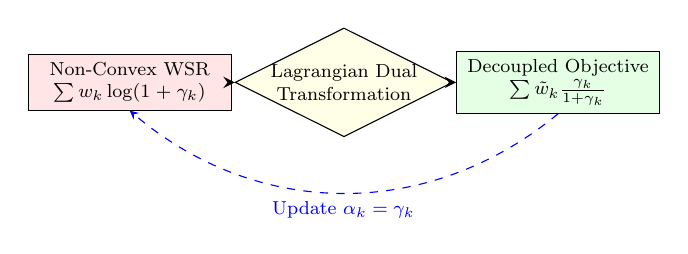
\begin{tikzpicture}[scale=0.85, transform shape,node distance=1.8cm, auto, >=stealth, font=\footnotesize]

    % Boxes
    \node[draw, rectangle, fill=red!10, text width=2.8cm, align=center] (original) {Non-Convex WSR \\ $\sum w_k \log(1+\gamma_k)$};

    \node[draw, diamond, fill=yellow!10, node distance=3.2cm, right of=original, aspect=2, inner sep=0pt, align=center] (dual) {Lagrangian Dual \\ Transformation};
    
    \node[draw, rectangle, fill=green!10, text width=2.8cm, align=center, node distance=3.2cm, right of=dual] (transformed) {Decoupled Objective \\ $\sum \tilde{w}_k \frac{\gamma_k}{1+\gamma_k}$};

    % Arrows
    \draw[->, thick] (original) -- (dual);
    \draw[->, thick] (dual) -- (transformed);
    
    % Auxiliary variable feedback - Wrapped in math mode $...$
    \draw[->, bend left=40, dashed, blue] (transformed.south) to node[below] {Update $\alpha_k = \gamma_k$} (original.south);

\end{tikzpicture}
\caption{Logic flow of the Lagrangian dual transformation. The logarithmic term is converted into a sum-of-ratios, introducing auxiliary variables $\alpha_k$ to track node-specific SINR.}
\label{fig:lagrangian_logic}
\end{figure}

\subsection{Multidimensional Quadratic Transform and Relational Linearization}
\label{subsec:quadratic_transform}

While the Lagrangian dual transformation addresses the logarithmic structure of the WSR, the resulting objective remains a sum-of-ratios problem where the optimization variables are coupled within the denominators of the SINR terms. To facilitate a structure-aware unfolding process, we apply the multidimensional quadratic transform to linearize these ratios into a tractable quadratic surface.

\subsubsection{Linearizing the Power Sub-Problem}
By fixing the reflecting coefficients $\mathbf{\Phi}$, we introduce a set of auxiliary variables $\boldsymbol{\beta} = [\beta_1, \dots, \beta_K]\trans \in \mathbb{C}^K$ to transform the fractional terms associated with power allocation. The objective function is recast into a quadratic form $f_2(\mathbf{p}, \boldsymbol{\beta})$ as:
\begin{equation}
\begin{aligned}
f_2(\mathbf{p}, \boldsymbol{\beta})
= \sum_{k=1}^K \Bigg(
&2 \operatorname{Re}\!\left\{
\beta_k^* \sqrt{\tilde{w}_k p_k}\, H_k
\right\} \\
&- |\beta_k|^2
\left(
\sum_{i\in\mathcal{U}} p_i |H_i|^2
+ \sigma^2
\right)
\Bigg).
\end{aligned}
\end{equation}
For a given power set $\mathbf{p}$, the optimal auxiliary variable $\beta_k^*$ that maximizes the local curvature is derived as:
\begin{equation}
    \beta_k^* = \frac{\sqrt{\tilde{w}_k p_k} H_k}{\sum_{i \in \mathcal{U}} p_i |H_i|^2 + \sigma^2}, \quad \forall k \in \mathcal{U}.
\end{equation}
This transformation is highly significant for our susequent unfolding architecture, as it identifies the interference-plus-noise floor as a normalizing factor for the learnable step-size.

\subsubsection{Linearizing the Phase-Shift Sub-Problem}
Symmetrically, by fixing the power $\mathbf{p}$, we optimize the reflecting coefficients $\boldsymbol{\Phi}$ by introducing the auxiliary vector $\boldsymbol{\epsilon} = [\epsilon_1, \dots, \epsilon_K]\trans \in \mathbb{C}^K$. Utilizing the cascaded channel notation $\mathbf{b}_{k,n}$ from Section \ref{subsubsec:channels}, the phase-centric objective is reformulated as:
\begin{equation}
    f_3(\boldsymbol{\Phi}, \boldsymbol{\epsilon}) = \sum_{k=1}^K 2 \text{Re} \left\{ \epsilon_k^* \sqrt{\tilde{w}_k p_k} H_k \right\} - \left( \sum_{k=1}^K |\epsilon_k|^2 \right) D(\boldsymbol{\Phi}),
\end{equation}
where $H_k$ represents the effective channel, and $D(\boldsymbol{\Phi}) = \sum_{i \in \mathcal{U}} p_i |H_i|^2 + \sigma^2$ denotes the total received power at the base station. Because $D(\boldsymbol{\Phi})$ is a global scalar common to all users, the quadratic penalty term is scaled by the aggregate weight $\sum_{k=1}^K |\epsilon_k|^2$. The optimal update for the auxiliary variable $\epsilon_k^*$ is given by:
\begin{equation}
    \epsilon_k^* = \frac{\sqrt{\tilde{w}_k p_k} \left( h_{d,k} + \sum_n x_{k,n} \mathbf{b}_{k,n}\herm \boldsymbol{\phi}_n \right)}{D(\boldsymbol{\Phi})}.
\end{equation}
Through these dual transformations, the originally intractable WSR problem is reduced to a sequence of quadratic sub-problems.

\subsection{The Alternating Optimization (AO) Benchmark}
\label{subsec:ao_benchmark}

The transformations established in Sections \ref{subsec:decoupling} and \ref{subsec:quadratic_transform} allow the orchestrator to solve the originally coupled WSR problem by iteratively updating one set of variables while keeping the others fixed. This iterative process serves as the performance upper bound and the source of the supervised labels used for the neural "warm-start" stage of our proposed framework.

\subsubsection{Optimal Power Allocation Laws}
\label{subsubsec:power_laws}

By fixing the auxiliary variables $\{\boldsymbol{\alpha}, \boldsymbol{\beta}, \boldsymbol{\epsilon}\}$ and the reflection manifold $\boldsymbol{\Phi}$, the optimization of the transmit power $\mathbf{p}$ reduces to maximizing the quadratic surrogate $f_2(\mathbf{p}, \boldsymbol{\beta})$ defined in Section \ref{subsec:quadratic_transform}. Since $f_2$ is a concave function with respect to the square root of the power, the stationary point can be found analytically.

The optimal power allocation $p_k^*$ for node $k$, while strictly observing the heterogeneous peak power budgets $P_k^{\text{peak}}$, is derived as:
\begin{equation}
    p_k^* = \min \left\{ P_k^{\text{peak}}, \frac{\tilde{w}_k \left( \text{Re} \{ \beta_k^* H_k \} \right)^2}{\left( |H_k|^2 \sum_{i=1}^K |\beta_i|^2 \right)^2} \right\}.
    \label{eq:power_update}
\end{equation}
Equation \eqref{eq:power_update} reveals a sophisticated \textit{Power Scaling} law. The denominator, which incorporates the sum of the magnitudes of all auxiliary variables $\beta_i$, acts as a global interference penalty. This implies that in a dense IoT environment, a node’s power allocation is not only determined by its own channel quality $H_k$ but is inversely proportional to the aggregate interference it causes to the rest of the network.

From a deep unfolding perspective, this closed-form solution is computationally efficient, involving only scalar operations. Consequently, for all three proposed paradigms—FONR, MASO, and TIAS—we implement this power update as a deterministic "Physics-Defined Layer," ensuring that the neural network strictly adheres to the peak power constraints of the IoT devices without requiring additional trainable parameters.


\subsubsection{Structure-Aware Reflection Optimization}
\label{subsubsec:reflection_optimization}

The final step in the alternating optimization loop involves the configuration of the reflection manifold $\boldsymbol{\Phi}$. By fixing the power allocation $\mathbf{p}$ and the auxiliary set $\{\boldsymbol{\alpha}, \boldsymbol{\beta}, \boldsymbol{\epsilon}\}$, the objective $f_3(\boldsymbol{\Phi}, \boldsymbol{\epsilon})$ defined in Section \ref{subsec:quadratic_transform} can be decomposed into $N$ independent sub-problems, one for each IRS $n \in \mathcal{N}$. 

Substituting the effective channel $H_k = h_{d,k} + \sum_n x_{k,n} \mathbf{b}_{k,n}\herm \boldsymbol{\phi}_n$ into the phase-centric objective and isolating the terms dependent on $\boldsymbol{\phi}_n$, the surrogate function for the $n$-th surface simplifies to a standard complex quadratic form:
\begin{equation}
    f_3(\boldsymbol{\phi}_n) = 2 \text{Re} \left\{ \mathbf{v}_n\herm \boldsymbol{\phi}_n \right\} - \boldsymbol{\phi}_n\herm \mathbf{A}_n \boldsymbol{\phi}_n + \text{const},
\end{equation}
where the Hermitian curvature matrix $\mathbf{A}_n \in \mathbb{C}^{M \times M}$ and the excitation vector $\mathbf{v}_n \in \mathbb{C}^{M \times 1}$ are explicitly derived as:
\begin{align}
    \mathbf{A}_n &= \left( \sum_{k=1}^K |\epsilon_k|^2 \right) \sum_{i=1}^K x_{i,n} p_i \mathbf{b}_{i,n} \mathbf{b}_{i,n}\herm, \\
    \mathbf{v}_n &= \sum_{i=1}^K x_{i,n} \left( \sqrt{\tilde{w}_i p_i} \epsilon_i - \left( \sum_{k=1}^K |\epsilon_k|^2 \right) p_i h_{d,i}^* \right) \mathbf{b}_{i,n}.
\end{align}
Setting the Wirtinger gradient $\nabla_{\boldsymbol{\phi}_n^*} f_3 = \mathbf{v}_n - \mathbf{A}_n \boldsymbol{\phi}_n$ to zero yields the unconstrained stationary point. Utilizing the relational cascaded channel $\mathbf{b}_{i,n}$ and the association parameter $x_{i,n}$, the unconstrained reflecting coefficient vector $\boldsymbol{\phi}_n^{\text{unc}}$ is determined by solving:
\begin{equation}
    \mathbf{A}_n \boldsymbol{\phi}_n^{\text{unc}} = \mathbf{v}_n.
    \label{eq:matrix_system}
\end{equation}

The classical unconstrained solution requires a direct matrix inversion, $\boldsymbol{\phi}_n^{\text{unc}} = \mathbf{A}_n^{-1} \mathbf{v}_n$. To satisfy the strict unit-modulus constraint of passive IRS hardware, this unconstrained analytical solution is directly projected onto the feasible continuous manifold (the unit circle):
\begin{equation}
    \phi_{n,m} = \frac{\phi_{n,m}^{\text{unc}}}{|\phi_{n,m}^{\text{unc}}|}, \quad \forall n \in \mathcal{N}, \forall m \in \mathcal{M}.
    \label{eq:projection}
\end{equation}

Crucially, projecting the unconstrained minimizer of a quadratic surrogate onto the unit circle does not mathematically yield the true constrained optimum. This operation is a low-complexity approximation that trades the strict monotonic convergence guarantees of exact fractional programming for computational tractability. Consequently, this update step serves as a highly effective local search heuristic rather than a theoretical upper bound. The objective of our proposed neural framework is to bypass the $\mathcal{O}(M^3)$ bottleneck of this exact matrix inversion while navigating the constrained manifold more effectively.

\subsection{Algorithmic Summary and Complexity Analysis}
\label{subsec:ao_summary}

The complete iterative procedure for the Alternating Optimization (AO) benchmark is summarized in Algorithm \ref{alg:teacher}. Rather than serving as an absolute theoretical upper bound, this algorithm acts as a "Teacher" that provides high-quality heuristic pseudo-labels against which the intelligent unfolding paradigms are initialized. By iteratively updating the auxiliary variables and the physical parameters ($\mathbf{p}, \boldsymbol{\Phi}$), the algorithm performs a directed local search through the parameter space.

\begin{algorithm}[H]
\caption{Classical AO-Based Local Search (The Pseudo-Label Generator)}
\label{alg:teacher}
\begin{algorithmic}[1]
\renewcommand{\algorithmicrequire}{\textbf{Input:}}
\renewcommand{\algorithmicensure}{\textbf{Output:}}
\REQUIRE Channels $\{h_{d,k}, \mathbf{b}_{k,n}, \mathbf{g}_n\}$, weights $w_k$, constraints $P_k^{\text{peak}}$.
\STATE \textbf{Initialize:} $x_{k,n}$ via max-gain heuristic, set $\mathbf{p}^{(0)}$ and $\boldsymbol{\Phi}^{(0)}$.
\REPEAT
    \STATE Update $\alpha_k$ for all $k \in \mathcal{U}$ using \eqref{eq:optimal_alpha}.
    \STATE Update $\beta_k$ for all $k \in \mathcal{U}$ via multidimensional quadratic transform.
    \STATE Update $\epsilon_k$ for all $k \in \mathcal{U}$ via multidimensional quadratic transform.
    \STATE \textbf{Power Allocation:} Update $p_k$ using \eqref{eq:power_update}.
    \STATE \textbf{Reflection Tuning:} Solve unconstrained $\boldsymbol{\phi}_n^{\text{unc}}$ for all $n \in \mathcal{N}$ via \eqref{eq:matrix_system}.
    \STATE Project $\boldsymbol{\phi}_n^{\text{unc}}$ onto the unit-modulus manifold using \eqref{eq:projection}.
\UNTIL{Convergence criteria $\frac{R^{(t+1)} - R^{(t)}}{R^{(t)}} < \eta$ is met.}
\ENSURE Heuristic power allocation $\mathbf{p}^*$ and phase-shift manifold $\boldsymbol{\Phi}^*$.
\end{algorithmic}
\end{algorithm}

\paragraph{Computational Complexity}
As established in Section \ref{subsubsec:reflection_optimization}, the computational cost of Algorithm \ref{alg:teacher} stems from three primary operations per iteration: evaluating the composite channels and auxiliary variables ($\mathcal{O}(K \cdot M)$), explicitly constructing the $M \times M$ coupling matrices $\mathbf{A}_n$ ($\mathcal{O}(K \cdot M^2)$), and performing the direct matrix inversions ($\mathcal{O}(N \cdot M^3)$). Consequently, the rigorous per-iteration complexity is bounded by $\mathcal{O}(K \cdot M^2 + N \cdot M^3)$. In a real-life IoT setting featuring massive IRS arrays, the cubic scaling of the matrix inversion ($\mathcal{O}(N \cdot M^3)$) severely dominates, introducing processing latency that easily exceeds the coherence time of the wireless channel.

\section{The Intelligent Unfolding Framework (IUF)}
\label{sec:unfolding_framework}

While the model-driven FP-AO benchmark derived in Section \ref{sec:math_baseline} provides a robust heuristic baseline, its practical utility is constrained by a \textit{Dual Bottleneck}: (i) the structural $\mathcal{O}(M^3)$ complexity of matrix inversions, and (ii) the convergence bottleneck of unpredictable, high-iteration counts.  

In our proposed IUF, we transform the iterative steps of Algorithm \ref{alg:teacher} into a deep feed-forward architecture with $L$ layers. Each layer $l \in \{1, \dots, L\}$ maps to a single FP-AO iteration, but replaces rigid mathematical operators with learnable neural components. This approach ensures deterministic latency and leverages the structural inductive bias of the fractional programming manifold to accelerate convergence.

\subsection{Architectural Progression: A Three-Stage Evolution}
\label{subsec:progression}

To systematically address the limitations of the FP-AO benchmark, we propose three distinct neural architectures. These are designed as an evolutionary progression, where each paradigm resolves a specific structural bottleneck of its predecessor:

\begin{itemize}
    \item \textbf{First-Order Neural Refinement (FONR):} Serving as our baseline learned first-order scheme, FONR demonstrates the immediate computational gains achieved by replacing the exact $\mathcal{O}(M^3)$ matrix inversion with a learned scalar step-size refinement. 
    \item \textbf{Manifold-Adaptive Step Optimization (MASO):} Acting as our primary element-wise architecture, MASO addresses FONR's susceptibility to ill-conditioned channels. It learns a diagonal preconditioner perfectly adapted to the anisotropic IRS curvature, thereby scaling the gradient appropriately for each individual reflecting element.
    \item \textbf{Topological Interference-Aware Search (TIAS):} Serving as our ultimate scalability and generalization extension, TIAS eliminates the fixed-dimensional MLP limitations of MASO. By executing the exact matrix-free computation of the surrogate gradient via bipartite message passing, TIAS achieves permutation-equivariant inference across arbitrary IRS and user dimensions.
\end{itemize}

This progression ($\text{FONR} \rightarrow \text{MASO} \rightarrow \text{TIAS}$) provides a comprehensive roadmap for transitioning from rigid analytical models to fully scalable, dimension-invariant neural orchestrators.

\subsection{Structural Synthesis: From Iterations to Layers}
\label{subsec:synthesis}

To ensure mathematical consistency, each layer $l$ of the IUF is designed as a direct architectural mapping of the AO steps defined in Algorithm \ref{alg:teacher}. The state of the network at any layer is represented by the tuple $\mathcal{S}^{(l)} = \{ \mathbf{p}^{(l)}, \boldsymbol{\Phi}^{(l)} \}$. The unfolding process proceeds as follows:

\begin{enumerate}
    \item \textbf{Physics-Defined Auxiliary Blocks:} Each layer begins by calculating the current auxiliary variables $\alpha_k^{(l)}$, $\beta_k^{(l)}$, and $\epsilon_k^{(l)}$ using the closed-form expressions derived in Section \ref{sec:math_baseline}. These are implemented as non-trainable, deterministic layers that "gate" the gradient flow according to the current interference floor.
    \item \textbf{Deterministic Resource Allocation:} The power allocation $p_k^{(l)}$ is updated via the optimal law in \eqref{eq:power_update}. By keeping this step deterministic, we ensure 100\% adherence to the heterogeneous power constraints $P_k^{\text{peak}}$ without the need for penalty-based loss functions.
    \item \textbf{Learnable Reflection Refinement:} The "hard" matrix inversion of \eqref{eq:matrix_system} is replaced by a neural mapping $\mathcal{F}_{\theta}(\cdot)$. This is the only component where trainable parameters $\theta$ are introduced, allowing the network to learn the acceleration of the manifold search.
\end{enumerate}

This modular approach preserves the \textit{Structural Inductive Bias} of fractional programming while offloading the most computationally expensive tasks to the neural domain.

\subsection{Architecture I: First-Order Neural Refinement (FONR)}
\label{subsec:fonr}

The FONR architecture, inspired by recent advances in gradient-based unrolling, is designed for extreme low-latency scenarios where even quadratic operations must be strictly bounded. Instead of solving the linear system directly, FONR implements the neural mapping $\mathcal{F}_{\theta}(\cdot)$ as a nested recursive refinement process. 

FONR recognizes the sensitivity of the WSR to phase-shift configurations by embedding an inner refinement loop within each outer optimization layer.

\subsubsection{Nested Recursive Refinement}
Each outer layer $l \in \{1, \dots, L\}$ of the FONR pipeline begins by updating the auxiliary variables and the transmit power $\mathbf{p}^{(l)}$ using the deterministic physics-defined layers. Subsequently, the network enters an inner refinement loop of depth $T$. For each inner step $t \in \{1, \dots, T\}$, the phase shifts are updated via a learned first-order step:
\begin{equation}
    \boldsymbol{\phi}_n^{(l, t)} = \mathcal{P}_{\mathcal{S}_{\phi}} \left( \boldsymbol{\phi}_n^{(l, t-1)} + \lambda^{(l)} \cdot \mathcal{N}_{\theta}^{(l)} \left( \nabla f_3^{(l, t-1)} \right) \right),
\end{equation}
where $\mathcal{P}_{\mathcal{S}_{\phi}}$ denotes the unconditional projection onto the unit-circle manifold $\mathcal{S}_{\phi} = \{ \phi \in \mathbb{C} \mid |\phi| = 1 \}$, and $\nabla f_3$ is the surrogate gradient synthesized from the quadratic transform:
\begin{equation}
    \nabla f_3^{(l, t-1)} = \mathbf{v}_n^{(l)} - \mathbf{A}_n^{(l)} \boldsymbol{\phi}_n^{(l, t-1)}.
\end{equation}

\subsubsection{Structural Inductive Bias and Scalar Weighting}
To minimize the parameter count—a critical requirement for power-constrained IoT gateways—we enforce weight sharing across all IRS elements. The neural operator $\mathcal{N}_{\theta}^{(l)}$ is implemented as a complex-valued scalar weighting, effectively allowing the network to learn the \textit{optimal momentum} of the gradient descent trajectory. 

By setting $T > 1$, the FONR architecture allows the intelligent orchestrator to "settle" the interference landscape through multiple first-order refinements before re-evaluating the power allocation in the next outer layer $l+1$. Crucially, to maximize computational efficiency, the inner gradient $\nabla f_3^{(l, t-1)}$ is evaluated using matrix-free operations. By computing the associative sequence $\mathbf{b}_{k,n} (\mathbf{b}_{k,n}\herm \boldsymbol{\phi}_n)$ directly from the interference sum, the network entirely bypasses the explicit $\mathcal{O}(K_n \cdot M^2)$ construction of the coupling matrix $\mathbf{A}_n$. 

Consequently, FONR reduces the computational complexity of the reflection update from the classical $\mathcal{O}(K \cdot M^2 + N \cdot M^3)$ down to a highly scalable $\mathcal{O}(T \cdot K \cdot M)$, achieving strict linear scaling with respect to the number of IRS elements.
% --- TikZ Illustration: NESTED FONR ARCHITECTURE ---
\begin{figure}[!t]
\centering
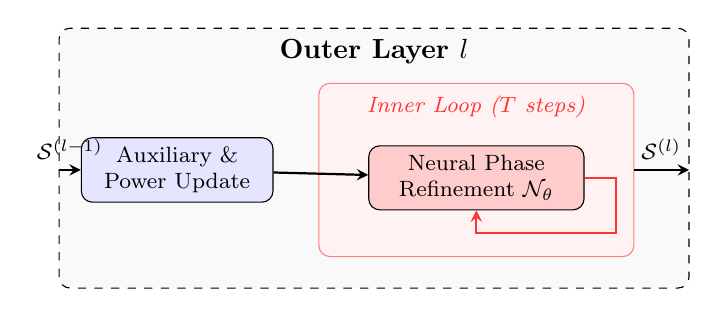
\begin{tikzpicture}[node distance=1.2cm, auto, >=stealth, font=\footnotesize]
    % Outer Box
    \draw[dashed, fill=gray!5, rounded corners] (-0.5,-1.5) rectangle (7.5,1.8);
    \node at (3.5, 1.5) [font=\bfseries] {Outer Layer $l$};

    % Deterministic Part
    \node[draw, rectangle, fill=blue!10, text width=2.2cm, align=center, rounded corners] (det) at (1,0) {Auxiliary \& \\ Power Update};

    % Inner Loop Box
    \draw[fill=red!5, draw=red!50, rounded corners] (2.8,-1.1) rectangle (6.8,1.1);
    \node[red!80] at (4.8, 0.8) {\textit{Inner Loop ($T$ steps)}};
    
    % Inner Step
    \node[draw, rectangle, fill=red!20, text width=2.5cm, align=center, rounded corners] (inner) at (4.8,-0.1) {Neural Phase \\ Refinement $\mathcal{N}_{\theta}$};

    % Connections
    \draw[->, thick] (-0.5,0) -- node[above] {$\mathcal{S}^{(l-1)}$} (det);
    \draw[->, thick] (det) -- (inner);
    \draw[->, thick, red!80] (inner.east) -- +(0.4,0) |- (4.8, -0.8) -- (inner.south);
    \draw[->, thick] (6.8,0) -- node[above] {$\mathcal{S}^{(l)}$} (7.5,0);

\end{tikzpicture}
\caption{The nested unfolding architecture of FONR. Each outer layer $l$ relies on deterministic physics blocks for power allocation, followed by an inner recursive loop of $T$ neural refinement steps to stabilize the reflection manifold.}
\label{fig:nested_fonr}
\end{figure}

\subsection{Architecture II: Manifold-Adaptive Step Optimization (MASO)}
\label{subsec:maso}

While the FONR architecture provides extreme computational efficiency, a single scalar step-size is highly susceptible to the ill-conditioned curvature of the quadratic surrogate. Because cascaded channel gains vary drastically across the massive IRS array, the optimization landscape exhibits highly anisotropic contours, causing standard first-order gradients to oscillate. To address this without resorting to full $\mathcal{O}(M^3)$ matrix inversions, Architecture II introduces a Manifold-Adaptive Step Optimization (MASO) strategy. Inspired by the nonhomogeneous quadratic transform, MASO acts as a neural preconditioner, learning element-wise adaptive step sizes that approximate the curvature of the analytical coupling matrix.

\subsubsection{Nonhomogeneous Curvature and Riemannian Preconditioning}
\label{subsubsec:neural_preconditioning}

In the classical analytical update derived in Section \ref{subsubsec:reflection_optimization}, the optimal reflection manifold is obtained via $\boldsymbol{\phi}_n^{\text{unc}} = \mathbf{A}_n^{-1} \mathbf{v}_n$. Here, the coupling matrix $\mathbf{A}_n$ acts as the Hermitian curvature matrix of the quadratic surrogate function $f_3$. A direct matrix inversion perfectly scales the update for every element, but at a prohibitive $\mathcal{O}(M^3)$ cost.

To bridge the gap between exact Newton-like methods and standard gradient descent while strictly respecting the feasible unit-circle set $\mathbb{T}^M = \{ \boldsymbol{\phi} : |\phi_m| = 1 \}$, MASO employs a \textit{manifold-adaptive} relaxation. Instead of performing an ambient-space projected-gradient step, MASO operates directly on the Riemannian manifold. The Euclidean Wirtinger gradient $\nabla_{\boldsymbol{\phi}^*} f_3^{(l)}$ is first projected onto the local tangent space to form the Riemannian gradient:
\begin{equation}
    \operatorname{grad}_{\mathbb{T}} f_3^{(l)} = \nabla_{\boldsymbol{\phi}^*} f_3^{(l)} - \text{Re} \left\{ \nabla_{\boldsymbol{\phi}^*} f_3^{(l)} \odot (\boldsymbol{\phi}_n^{(l)})^* \right\} \odot \boldsymbol{\phi}_n^{(l)}.
\end{equation}

MASO seeks a multidimensional step-size vector $\boldsymbol{\lambda}_n^{(l)} \in \mathbb{R}_+^M$ to precondition this tangent direction. By learning this vector dynamically, the network updates the phase shifts along the tangent space, followed by a manifold retraction:
\begin{equation}
    \boldsymbol{\phi}_n^{(l+1)} = \frac{\boldsymbol{\phi}_n^{(l)} + \boldsymbol{\lambda}_n^{(l)} \odot \operatorname{grad}_{\mathbb{T}} f_3^{(l)}}{\left| \boldsymbol{\phi}_n^{(l)} + \boldsymbol{\lambda}_n^{(l)} \odot \operatorname{grad}_{\mathbb{T}} f_3^{(l)} \right|}.
    \label{eq:maso_update}
\end{equation}
This formulation allows the network to adaptively precondition the Riemannian gradient step based on local channel quality, accelerating convergence without requiring dense $\mathcal{O}(M^3)$ matrix inversions.

\subsubsection{MLP-Driven Step Prediction and the Dimensionality Bottleneck}
\label{subsubsec:maso_mlp}

To map the complex interference environment to the optimal nonhomogeneous step size, MASO employs a Multi-Layer Perceptron (MLP) within each unrolled layer. The neural preconditioner must observe both the physical channel conditions and the current mathematical state of the optimization loop. 

For the $n$-th IRS at layer $l$, we construct an input feature vector $\mathbf{z}_n^{(l)}$ by concatenating the real and imaginary components of the local environment variables. These include the cascaded channel vectors $\mathbf{b}_{k,n}$ for all clustered users ($x_{k,n}=1$), the current reflection manifold $\boldsymbol{\phi}_n^{(l)}$, and the auxiliary interference metrics $\boldsymbol{\epsilon}^{(l)}$. The adaptive step-size vector is generated via:
\begin{equation}
    \boldsymbol{\lambda}_n^{(l)} = \text{Softplus} \left( \Psi_{\theta_n}^{(l)} (\mathbf{z}_n^{(l)}) \right),
\end{equation}
where $\Psi_{\theta_n}^{(l)}(\cdot)$ denotes the MLP mapping parameterized by weights and biases $\theta_n$, and the Softplus activation ensures that the predicted step sizes remain strictly positive to maintain gradient ascent stability.

By replacing the exact matrix inversion with a neural forward pass, MASO significantly reduces the computational overhead of the reflection update. The analytical gradient $\nabla f_3^{(l)}$ can be evaluated using matrix-free associative operations, requiring $\mathcal{O}(K \cdot M)$ complexity per surface. Subsequently, passing the feature vector through the MLP—assuming hidden layer dimensions scale proportionally to the array size $M$—requires dense matrix-vector multiplications that incur an $\mathcal{O}(M^2)$ computational cost. Consequently, MASO bounds the overall per-layer complexity to $\mathcal{O}(K \cdot M + M^2)$. This represents a massive reduction from the $\mathcal{O}(K \cdot M^2 + M^3)$ cost of the classical exact inversion, though the $\mathcal{O}(M^2)$ MLP overhead can still be noticeable for extremely large IRS arrays.

\paragraph{The Dimensionality Bottleneck} 
While MASO resolves the anisotropic curvature problem and eliminates the need for nested inner loops, it introduces a severe architectural constraint. Standard MLPs mandate a strictly fixed input dimensionality. In \eqref{eq:maso_update}, the size of the feature vector $\mathbf{z}_n^{(l)}$ is inherently tied to the number of users $K$ clustered around the IRS. 

In a dynamic IoT environment, devices frequently enter sleep modes, move between coverage zones, or alter the cluster mapping $x_{k,n}$. A change in the active user count alters the dimension of $\mathbf{z}_n^{(l)}$, instantly rendering the pre-trained MASO weights incompatible. While zero-padding can artificially fix the dimension, it degrades the network's predictive accuracy. This lack of \textit{topological permutation invariance} necessitates an architecture capable of learning dynamic relational graphs, motivating the introduction of our final paradigm.

% --- TikZ Illustration: MASO Layer Architecture ---
\begin{figure}[!t]
\centering
\begin{tikzpicture}[node distance=1.5cm, auto, >=stealth, font=\footnotesize]
    
    % Inputs
    \node (phi_in) at (0, 1.5) {$\boldsymbol{\phi}_n^{(l)}$};
    \node (features) at (0, -1.5) [align=center] {Local Features \\ $\mathbf{b}_{k,n}, \epsilon_k^{(l)}$};

    % Mathematical Gradient
    \node[draw, rectangle, fill=blue!5, text width=2cm, align=center, rounded corners] (grad) at (3, 1.5) {Analytical Gradient \\ $\nabla f_3^{(l)}$};
    
    % Neural Preconditioner (MLP)
    \node[draw, rectangle, fill=purple!10, text width=2.2cm, align=center, rounded corners] (mlp) at (3, -1.5) {Neural MLP \\ $\Psi_{\theta_n}^{(l)}}$};
    
    % Outputs of blocks
    \node (lambda) at (5.5, -1.5) {$\boldsymbol{\lambda}_n^{(l)}$};
    
    % Hadamard Product
    \node[draw, circle, fill=yellow!20, inner sep=2pt] (hadamard) at (5.5, 1.5) {$\odot$};
    
    % Summation
    \node[draw, circle, inner sep=2pt] (sum) at (7, 1.5) {$+$};
    
    % Output
    \node (phi_out) at (8.5, 1.5) {$\boldsymbol{\phi}_n^{(l+1)}$};

    % Routing
    \draw[->, thick] (phi_in) -- (grad);
    \draw[->, thick] (features) -- (mlp);
    
    % Cross routing for MLP to see phi
    \draw[->, dashed, gray] (1, 1.5) |- (mlp.west);
    
    \draw[->, thick] (grad) -- (hadamard);
    \draw[->, thick] (mlp) -- (lambda);
    \draw[->, thick] (lambda) -- (hadamard);
    
    \draw[->, thick] (hadamard) -- (sum);
    \draw[->, thick, bend left=35] (phi_in.north) to (sum.north);
    \draw[->, thick] (sum) -- node[above] {Proj.} (phi_out);

\end{tikzpicture}
\caption{Architecture of the MASO layer. The MLP acts as a neural preconditioner, learning an element-wise step-size vector $\boldsymbol{\lambda}_n$ to optimally scale the analytical gradient without matrix inversion.}
\label{fig:maso_architecture}
\end{figure}


\subsection{Architecture III: Topological Interference-Aware Search (TIAS)}
\label{subsec:tias}

While the MASO architecture successfully circumvents the $\mathcal{O}(M^3)$ matrix inversion bottleneck, its reliance on an MLP imposes a severe structural rigidity: the input feature dimension is strictly fixed. Consequently, MASO relies on layer-specific parameters that fail to generalize across varying problem sizes or iteration numbers. If a new IoT device joins the network, the dimension of the interference feature vector changes, instantly rendering the pre-trained MASO weights incompatible. 

To overcome this dimensionality bottleneck and achieve zero-shot generalization, we propose Architecture III: Topological Interference-Aware Search (TIAS). Inspired by structure-aware graph neural networks, TIAS directly unfolds the classical fractional programming framework into a topological bipartite graph. By modeling the optimization variables as nodes and the interference coupling as edges, TIAS achieves strict permutation and dimension invariance.

\subsubsection{Bipartite Graph Construction from Heuristic Association}
\label{subsubsec:tias_graph}

The standard single-variable quadratic form of the phase-shift subproblem can be naturally mapped onto a bipartite graph $\mathcal{G}^{(l)} = (\mathcal{V}, \mathcal{E})$. The vertex set $\mathcal{V} = \mathcal{V}_{\text{obs}} \cup \mathcal{V}_{\text{var}}$ consists of two disjoint sets of nodes:
\begin{itemize}
    \item \textbf{Observation Nodes ($\mathcal{V}_{\text{obs}}$):} Representing the $K$ active IoT users. Each node $k \in \mathcal{V}_{\text{obs}}$ maintains a state vector containing its local interference floor and the auxiliary variable $\epsilon_k^{(l)}$.
    \item \textbf{Variable Nodes ($\mathcal{V}_{\text{var}}$):} Representing the $N \times M$ passive reflecting elements distributed across the network. Each node $(n,m) \in \mathcal{V}_{\text{var}}$ holds its current continuous phase-shift value $\phi_{n,m}^{(l)}$.
\end{itemize}

The topology of this graph is not learned; rather, the edge set $\mathcal{E}$ is constructed directly from the externally imposed heuristic association parameter $x_{k,n}$ defined in Section \ref{subsec:constraints}. A directed edge $e_{k \to (n,m)}$ exists if and only if user $k$ has been pre-clustered to the $n$-th IRS:
\begin{equation}
    \mathcal{E} = \left\{ (k, (n,m)) \mid x_{k,n} = 1, \forall k \in \mathcal{U}, \forall n \in \mathcal{N}, m \in \mathcal{M} \right\}.
\end{equation}
The feature of each active edge is parameterized by the scalar cascaded channel coefficient $b_{k,n,m}$. 

While the topology remains fixed during the optimization loop for a given time frame, the graph representation is highly advantageous for dynamic IoT environments. If an IoT user enters a sleep state or is re-clustered by the base station heuristic in a subsequent time frame, the binary state $x_{k,n}$ flips, and the corresponding edges are updated. Because Graph Neural Networks process data by aggregating information along active edges rather than traversing fixed-size matrices, TIAS effortlessly operates on this newly constructed topology without requiring any alterations to its underlying neural architecture.

\subsubsection{Structure-Aware Neural Message Passing}
\label{subsubsec:tias_message_passing}

To execute the nonhomogeneous fractional programming update without constructing the full $\mathcal{O}(M^3)$ coupling matrix $\mathbf{A}_n$, TIAS simulates the quadratic optimization through bidirectional local message passing on the bipartite graph $\mathcal{G}^{(l)}$. Rather than acting as a complete global interference graph—since global coupling occurs centrally through the SINR denominator—this structure functions as a user-IRS-element bipartite computational graph specifically designed for evaluating the phase-surrogate gradient. The execution of a single TIAS layer proceeds in three sequential phases:

\paragraph{Phase 1: Variable-to-Observation Phase-Shift Aggregation}
Before a user node can evaluate its local gradient contribution, it must observe the current reflection manifold. Each variable node $(n,m) \in \mathcal{V}_{\text{var}}$ broadcasts its current state along the active edges. The observation node $k \in \mathcal{V}_{\text{obs}}$ aggregates these incoming messages to compute the instantaneous reflected channel scalar:
\begin{equation}
    \psi_{k,n}^{(l)} = \sum_{m=1}^M x_{k,n} b_{k,n,m}^* \phi_{n,m}^{(l)}.
\end{equation}
Using this aggregated state, the observation node synthesizes a unified scalar interference feature $c_k^{(l)}$ that precisely captures its contribution to the analytical gradient:
\begin{equation}
    c_k^{(l)} = \sqrt{\tilde{w}_k p_k^{(l)}} \epsilon_k^{(l)} - \Xi^{(l)} p_k^{(l)} \left( h_{d,k}^* + \psi_{k,n}^{(l)} \right),
\end{equation}
where $\Xi^{(l)} = \sum_{i=1}^K |\epsilon_i^{(l)}|^2$ acts as the global scaling penalty derived in Section \ref{sec:math_baseline}.

\paragraph{Phase 2: Observation-to-Variable Interference Distribution}
Once the local gradient scalar is synthesized, the observation node transmits it back across the active edges. The multi-dimensional message $\mathbf{m}_{k \to (n,m)}^{(l)}$ sent to the $(n,m)$-th variable node explicitly encodes this gradient step alongside the local channel magnitude:
\begin{equation}
    \mathbf{m}_{k \to (n,m)}^{(l)} = \Big[ b_{k,n,m} c_k^{(l)}, \; |b_{k,n,m}|^2 \Big]\trans.
\end{equation}
The variable node then aggregates these incoming messages from its active neighborhood $\mathcal{N}(n,m)$ using a permutation-invariant sum-pooling operator to form its comprehensive state vector:
\begin{equation}
    \mathbf{u}_{n,m}^{(l)} = \sum_{k \in \mathcal{N}(n,m)} \mathbf{m}_{k \to (n,m)}^{(l)}.
\end{equation}
By utilizing this bidirectional structure, the aggregated state $\mathbf{u}_{n,m}^{(l)}$ perfectly encapsulates the $m$-th element of the exact analytical gradient vector $\nabla f_3^{(l)}$, inherently avoiding the construction of any $M \times M$ dense matrices.

\paragraph{Phase 3: Node State Refinement}
By utilizing this bidirectional structure, the aggregated state $\mathbf{u}_{n,m}^{(l)}$ perfectly encapsulates the $m$-th element of the exact analytical gradient vector $\nabla f_3^{(l)}$. Ultimately, TIAS computes the FP surrogate gradient through permutation-invariant message passing without explicitly constructing $\mathbf{A}_n$, and then applies a learned node-wise update function $\mathcal{F}_{\text{GNN}}$ to act as a local neural preconditioner:
\begin{equation}
    \phi_{n,m}^{(l+1)} = \frac{\phi_{n,m}^{(l)} + \mathcal{F}_{\text{GNN}} \big( \mathbf{u}_{n,m}^{(l)}, \phi_{n,m}^{(l)} ; \mathbf{\Theta}_{\text{shared}} \big)}{\left| \phi_{n,m}^{(l)} + \mathcal{F}_{\text{GNN}} \big( \mathbf{u}_{n,m}^{(l)}, \phi_{n,m}^{(l)} ; \mathbf{\Theta}_{\text{shared}} \big) \right|}.
    \label{eq:tias_node_update}
\end{equation}
The unconditional unit-circle projection ensures strict physical feasibility for passive reflecting elements. Because the message passing relies exclusively on local neighborhood aggregation, the computational complexity scales linearly with the number of active edges, achieving a strict $\mathcal{O}(|\mathcal{E}|) \approx \mathcal{O}(K_{\text{active}} \cdot M)$ complexity per layer.

\subsubsection{Parameter Sharing and Zero-Shot Generalization}
\label{subsubsec:tias_generalization}

The most profound architectural advantage of TIAS over both the classical FP baseline and the MASO paradigm lies in its parameter efficiency and topological flexibility. In MASO (and standard DeepFP variants), the neural preconditioner requires distinct weight matrices for each unrolled layer $l$, leading to an expanding parameter footprint. Furthermore, because the input feature dimension is strictly bound to the active user count, MASO models are confined to the specific network density on which they were trained.

TIAS shatters this dimensionality bottleneck by enforcing strict weight sharing across both the spatial and temporal domains. Spatially, the parameter set $\mathbf{\Theta}_{\text{shared}}$ of the neural update function $\mathcal{F}_{\text{GNN}}$ is applied universally across all $N \times M$ variable nodes. Temporally, the exact same neural weights are reused across all $L$ layers of the unrolled network. This design inherently mimics the classical FP algorithm, where the fundamental mathematical rules of the quadratic update remain constant regardless of the specific reflecting element being optimized or the current iteration number.

Consequently, the size of $\mathbf{\Theta}_{\text{shared}}$ is entirely independent of the number of users $K$, the total number of IRS elements $M$, and the number of unrolled layers $L$. Because the GNN aggregates interference through the sum-pooling of local edge messages, the input dimension to $\mathcal{F}_{\text{GNN}}$ is always fixed (determined by the length of the aggregated state $\mathbf{u}_{n,m}^{(l)}$), regardless of how many users are actively clustered to the surface.

This structural dimension-invariance enables size-generalizable inference for the intelligent orchestrator. The TIAS architecture can be trained offline using a highly constrained, sparse simulation environment (e.g., small-scale IRS arrays serving a minimal number of devices). Once the optimal message-passing weights $\mathbf{\Theta}_{\text{shared}}$ are learned, the fixed parameter count and permutation equivariance facilitate zero-shot transfer across varying network sizes. The model can be deployed online to manage a dense, massive IoT environment featuring dynamic user clustering and fluid edge topologies, bypassing the dimensionality bottleneck. By directly unfolding the computational graph of the fractional programming objective, TIAS achieves the deterministic $\mathcal{O}(|\mathcal{E}|)$ latency of neural networks while inheriting the structural scalability of classical analytical optimization.

% --- TIAS Bipartite Graph Architecture ---
    \begin{figure}[h]
        \centering
        \includegraphics[width=\columnwidth]{tias_architecture}
        \caption{Bipartite computational graph topology of the TIAS architecture. The dynamic clustering heuristic ($x_{k,n}$) acts as a gating mechanism for the network edges. Active observation nodes ($k$) transmit structured interference messages to the IRS variable nodes $(n,m)$, which aggregate the data and update their continuous phase shifts using a universally shared GNN weight matrix $\mathbf{\Theta}_{\text{shared}}$. A final differentiable layer ensures rigorous constraint mapping.}
        \label{fig:tias_architecture}
    \end{figure}

% --- Section V: Hybrid Training Protocol ---
\section{Hybrid Training Protocol}
\label{sec:training_protocol}

Training deep unrolled architectures for highly non-convex WSR maximization requires a careful balance between convergence stability and the exploration of the complex parameter space. Relying exclusively on unsupervised learning from a random initialization often traps the network in poor local optima, whereas pure imitation encourages the network to reproduce the teacher solutions and may limit its ability to exploit solutions outside the teacher-generated training manifold. 

To address this, we propose a two-stage hybrid training protocol that synthesizes the reliability of model-driven optimization with the unbounded exploration capacity of data-driven learning. The proposed training regime consists of a supervised warm-start phase designed to achieve rapid convergence and robust initialization, seamlessly followed by an unsupervised fine-tuning phase where the network learns to directly maximize the actual physical objective. By applying this unified training umbrella across the FONR, MASO, and TIAS architectures, we ensure that the structural inductive biases of each network are optimally calibrated to the multi-user interference landscape.

\subsection{Stage I: Supervised Warm-Start (Imitation Learning)}
\label{subsec:stage_1_supervised}

The first stage of our protocol employs supervised learning to ensure rapid convergence and establish a robust initialization for the neural weights. Because the WSR maximization problem is highly non-convex and NP-hard, randomly initialized neural networks are prone to gradient vanishing or becoming trapped in severe local optima. By treating the converged outputs of the model-driven FP-AO benchmark as pseudo-optimal teacher solutions rather than absolute ground truth, we force the network into a stable and high-performing region of the parameter space before attempting to maximize the physical objective directly.

\subsubsection{Label Generation}
For a given training dataset comprising randomly generated channel realizations $\mathcal{H} = \{ h_{d,k}, \mathbf{b}_{k,n} \}$, we first execute Algorithm \ref{alg:teacher} (The Teacher) offline until strict convergence criteria are met. This produces the pseudo-optimal labels for the system: the transmit power allocation $\mathbf{p}^*$ and the passive reflection manifold $\boldsymbol{\Phi}^*$. Because the power allocation $\mathbf{p}^{(l)}$ in our unfolded architectures is inherently determined by the deterministic physics-defined layer defined in \eqref{eq:power_update}, the neural networks strictly focus on learning the phase-shift mapping from these teacher solutions.

\subsubsection{Phase Alignment Loss Formulation}
During this warm-start phase, the networks are trained to imitate the Teacher algorithm. However, applying a standard Mean Squared Error (MSE) Euclidean distance to unit-modulus variables is sub-optimal, as it does not inherently respect the periodic geometry of the phase manifold. Instead, we formulate the supervised loss using cosine similarity to strictly measure the angular distance between the neural network's final layer output $\phi_{n,m}^{(L)}$ and the Teacher's heuristic phase-shift label $\phi_{n,m}^*$. 

For a specific channel realization sample, the phase alignment loss is defined as:
\begin{equation}
    \mathcal{L}_{\text{Supervised}} = \frac{1}{N M} \sum_{n=1}^N \sum_{m=1}^M \left( 1 - \text{Re} \left\{ \phi_{n,m}^{(L)} (\phi_{n,m}^*)^* \right\} \right),
\end{equation}
where $(\phi_{n,m}^*)^*$ denotes the complex conjugate of the Teacher's target phase. This angular loss gracefully mitigates phase wrapping boundaries and ensures a smooth gradient landscape directly on the unit circle. 

This supervised warm-start acts as a form of behavioral cloning, allowing the structural parameters $\theta$ (in FONR/MASO) or $\mathbf{\Theta}_{\text{shared}}$ (in TIAS) to rapidly approximate the $\mathcal{O}(M^3)$ matrix inversion behavior at a fraction of the computational cost, seamlessly preparing the network for the subsequent WSR-driven fine-tuning stage.

\subsection{Stage II: Unsupervised Fine-Tuning (Physics-Driven)}
\label{subsec:stage_2_unsupervised}

While the supervised warm-start establishes a reliable and stable baseline, the classical AO algorithm remains susceptible to converging to sub-optimal stationary points due to the severe non-convexity of the multi-user interference landscape. To enable the unfolded architectures to potentially surpass the performance ceiling of the Teacher algorithm, the second stage of our protocol transitions to an unsupervised fine-tuning regime . We hypothesize that this unsupervised fine-tuning stage allows the network to discover phase-shift configurations that escape the rigid alternating structure of the AO baseline; empirical validation of this hypothesis is provided in Section \ref{sec:numerical_results}. In this phase, the neural network bypasses the algorithmic pseudo-labels and learns to directly optimize the physical performance metrics.

\subsubsection{Composite Loss Formulation}
We formulate a composite unsupervised loss function to drive this fine-tuning stage. The primary objective is to maximize the true system capacity, which translates to minimizing the negative batch WSR . However, directly backpropagating through the highly non-linear, coupled fractional WSR expression can occasionally lead to gradient instability during the early fine-tuning epochs. 

To mitigate this and provide a smoother optimization trajectory, we introduce a secondary stabilization term derived from the analytical quadratic surrogate function, $f_3(\boldsymbol{\Phi}, \boldsymbol{\epsilon})$, formulated in Section \ref{sec:math_baseline}. For a given training batch $\mathcal{B}$ comprising $|\mathcal{B}|$ independent channel realizations, the composite unsupervised loss is defined as a convex combination of the two objectives:
\begin{equation}
    \mathcal{L}_{\text{Unsup}} = \frac{1}{|\mathcal{B}|} \sum_{\mathcal{H} \in \mathcal{B}} \Big( -\alpha \cdot R(\mathbf{p}^{(L)}, \boldsymbol{\Phi}^{(L)}) - (1-\alpha) \cdot f_3(\boldsymbol{\Phi}^{(L)}, \boldsymbol{\epsilon}^{(L)}) \Big),
    \label{eq:composite_loss}
\end{equation}
where $R(\mathbf{p}^{(L)}, \boldsymbol{\Phi}^{(L)})$ is the achieved physical WSR at the final layer $L$, and $\alpha \in [0, 1]$ is a tunable hyperparameter that balances the contribution of the physical rate versus the surrogate function. By employing the negative surrogate $-f_3$, we ensure that gradient descent consistently pushes the network along the fractional programming ascent direction.

\subsubsection{Surrogate-Driven Stabilization and Auxiliary Evaluation}
Crucially, within this loss formulation, the auxiliary variable vector $\boldsymbol{\epsilon}^{(L)}$ is \textit{not} treated as a free, learnable parameter. Instead, it is computed deterministically from the current network outputs $(\mathbf{p}^{(L)}, \boldsymbol{\Phi}^{(L)})$ using the exact closed-form optimal update defined in Section \ref{sec:math_baseline}. 

By evaluating $\boldsymbol{\epsilon}^{(L)} = \boldsymbol{\epsilon}^*(\mathbf{p}^{(L)}, \boldsymbol{\Phi}^{(L)})$, the term $\nabla_{\boldsymbol{\Phi}} f_3(\boldsymbol{\Phi}^{(L)}, \boldsymbol{\epsilon}^*)$ remains perfectly aligned with the theoretical FP ascent direction. Consequently, auto-differentiation correctly backpropagates through this deterministic mapping, allowing the surrogate function to act as a mathematical "physics anchor." This composite formulation ensures that the data-driven exploration remains physically grounded, allowing the FONR, MASO, and TIAS architectures to discover highly efficient phase-shift manifolds while avoiding early-epoch instability.

\subsection{Deep Supervision and Layer-Wise Cumulative Loss}
\label{subsec:deep_supervision}

In standard deep unfolding paradigms, the loss function is typically evaluated only at the output of the final layer $L$. However, backpropagating gradients through a deep unfolded sequence solely from the final output can lead to the vanishing gradient problem, causing unstable updates in the earlier layers and ultimately degrading the overall convergence speed. 

To overcome this, we incorporate a deep supervision mechanism by formulating a layer-wise cumulative loss. Rather than applying the objective function exclusively to the final state $\mathcal{S}^{(L)} = \{ \mathbf{p}^{(L)}, \boldsymbol{\Phi}^{(L)} \}$, the loss is calculated as a weighted sum of the performance achieved at \textit{every} intermediate layer $l \in \{1, \dots, L\}$. Expanding upon the fine-tuning stage, the cumulative unsupervised loss $\mathcal{L}_{\text{Cum-Unsup}}$ is expressed as:
\begin{equation}
    \mathcal{L}_{\text{Cum-Unsup}} = \sum_{l=1}^L \rho^{(l)} \mathcal{L}_{\text{Unsup}}^{(l)},
\end{equation}
where $\mathcal{L}_{\text{Unsup}}^{(l)}$ is the composite unsupervised loss (defined in \eqref{eq:composite_loss}) evaluated using the network state at layer $l$, and $\rho^{(l)} > 0$ is a layer-specific discount factor. Typically, $\rho^{(l)}$ is chosen to increase monotonically with $l$ to ensure the network prioritizes the ultimate performance at the final layer while still penalizing early-layer degradation.

This deep supervision encourages each intermediate layer to produce a high-quality feasible solution and provides direct gradient signals to earlier layers. By explicitly routing the physical objective gradient to every step of the unfolded process, this technique significantly accelerates the training convergence of the FONR, MASO, and TIAS architectures while ensuring layer-to-layer stability.

\subsection{End-to-End Differentiability and Phase Parameterization}
\label{subsec:differentiability}

A fundamental challenge in training unrolled optimization networks for RIS-aided systems is ensuring that gradients can backpropagate through the physical hardware constraints. If the projection operator is non-differentiable or piecewise, the gradient flow is severed. 

To guarantee end-to-end differentiability and strict physical feasibility without relying on unstable Cartesian projection heuristics, we bypass complex-domain normalization entirely. Instead, we reparameterize the optimization space into the real angular domain. The strict unit-modulus constraint for passive RIS elements ($|\phi_{n,m}| = 1$) is unconditionally enforced by letting the neural network output a real-valued phase increment $\Delta\theta_{n,m}^{(l)}$ at each layer. The continuous phase state is updated via:
\begin{equation}
    \theta_{n,m}^{(l+1)} = \theta_{n,m}^{(l)} + \Delta\theta_{n,m}^{(l)},
\end{equation}
which is then deterministically mapped to the complex reflection coefficient using the Euler formulation:
\begin{equation}
    \phi_{n,m}^{(l+1)} = e^{j\theta_{n,m}^{(l+1)}}.
\end{equation}

Because the complex exponential is infinitely differentiable everywhere and inherently bounds the magnitude to exactly $1$, it functions as a transparent, mathematically flawless constraint mapping during training. This exponential mapping ensures that the analytical gradients propagate seamlessly through the FONR inner loops, the MASO preconditioning MLPs, and the TIAS bipartite message-passing edges. Consequently, standard auto-differentiation frameworks can optimize the structural network weights directly over the Riemannian manifold without encountering numerical singularities.

% --- Section VI: Numerical Results ---
\section{Numerical Results}
\label{sec:numerical_results}

This section rigorously evaluates the performance, computational scalability, and generalization capabilities of the proposed Intelligent Unfolding Framework (IUF). We benchmark the three neural architectures—First-Order Neural Refinement (FONR), Manifold-Adaptive Step Optimization (MASO), and Topological Interference-Aware Search (TIAS)—against the model-driven Alternating Optimization (AO) baseline. To ensure statistical validity and reproducibility, all evaluations are conducted over a large, independently generated test dataset rather than a limited sample pool.

\subsection{Simulation Environment and Baselines}
\label{subsec:sim_setup}

We consider a multi-IRS uplink IoT network consisting of a single-antenna base station, $N=2$ intelligent reflecting surfaces, and $K$ single-antenna IoT devices. The devices are partitioned into two heterogeneous classes: Type-I Critical Reporting Nodes (CRN) with a peak transmit power of 20 dBm and higher priority weights $\omega_k \in \{0.90, 0.80, 0.85\}$, and Type-II Periodic Monitoring Nodes (PMN) with a peak transmit power of 10 dBm and lower priority weights $\omega_k \in \{0.30, 0.20, 0.25\}$. 

The noise power is set to $\sigma^2 = -90$ dBm. Large-scale path loss follows the model $128.1 + 37.6 \log_{10}(d/1000)$ with an additional 20 dB NLOS penalty on the direct links and 8 dB log-normal shadowing. Small-scale fading on the IRS-related links is Rician with factor $\kappa = 10$, while the direct links are Rayleigh. User locations are drawn uniformly inside a disk of radius 20 m; the IRSs are fixed at predetermined locations. 

Each unfolded network comprises $L=10$ layers. The neural networks are trained using the Adam optimizer with a constant learning rate of $0.1$. To guarantee the rigor of our claims regarding zero-shot generalization and optimality gaps, we discard small-sample averaging in favor of large-scale statistical testing. The comprehensive system and network hyperparameters are summarized in Table \ref{tab:sim_parameters}.

\begin{table}[ht]
\centering
\caption{Simulation Parameters and Network Hyperparameters}
\label{tab:sim_parameters}
\begin{tabular}{@{}ll@{}}
\toprule
\textbf{Parameter} & \textbf{Value} \\ \midrule
Number of IRSs ($N$), Default Elements ($M$) & 2, 80 \\
Number of Active Users ($K$) & 6 (Training), $10, 15, \dots, 60$ (Test) \\
Training / Validation / Test Samples & $10^4$ / $10^3$ / $10^3$ (Independent) \\
Unfolded Layers ($L$) & 10 \\
Optimizer & Adam ($\text{LR} = 0.1$, constant) \\
Training Epochs & 50 (Supervised), 150 (Unsupervised) \\
FP-AO Stopping Criterion & $\Delta R / R < 10^{-5}$ or Max $100$ Iters \\
\bottomrule
\end{tabular}
\end{table}

\subsection{Algorithmic Convergence and Optimality Gap}
\label{subsec:convergence}

To rigorously evaluate the optimization quality, we first decouple the algorithmic convergence (measured in discrete steps) from the practical convergence (measured in wall-clock latency). Fig. \ref{fig:convergence}(a) traces the WSR evolution against the respective algorithmic step—FP-AO iterations for the benchmark, and unfolded layers for the neural architectures. Starting from an identical random feasible initialization, the neural architectures successfully approximate the fixed point of the fractional-programming iteration, recovering approximately 90\% of the eventual steady-state WSR gain by the fourth layer, exceeding 96\% by the sixth layer, and surpassing 98\% by the eighth layer, after which all four curves visibly flatten and become statistically indistinguishable. 

However, mapping an FP-AO iteration directly to a neural network layer on the same axis obscures the true computational advantage. Fig. \ref{fig:convergence}(b) rectifies this by plotting the WSR convergence against actual wall-clock inference time. Because a single FP-AO iteration executes an exact $\mathcal{O}(M^3)$ matrix inversion, its time-domain convergence is severely penalized. Conversely, the matrix-inversion-free updates of the proposed architectures allow them to execute their entire forward passes in a fraction of the time required for a single FP-AO step. TIAS, in particular, reaches approximately 98\% of AO's converged steady-state WSR within the same wall-clock budget ($\approx 0.85$ ms) that AO requires just to complete its \emph{first} phase-shift update, and it crosses 99\% of that steady-state value by $\approx 1$ ms -- nearly an order of magnitude before AO itself converges at $\approx 7.9$--$8.8$ ms.
\begin{figure}[htbp]
	\centering
	\begin{subfigure}[b]{0.5\textwidth}
		\centering
		\caption{}
		\includegraphics[width=\textwidth]{WSR_vs_iteration.png}
	\end{subfigure}
	\hfill
	\begin{subfigure}[b]{0.5\textwidth}
		\centering
		\caption{}
		\includegraphics[width=\textwidth]{WSR_vs_wall_clock.png}
	\end{subfigure}
	\caption{Convergence profiles of the evaluated algorithms. (a) WSR versus algorithmic step (FP-AO iterations or unfolded layers). Shaded regions denote the 95\% confidence intervals over $80$ independent test channel realizations. (b) WSR versus actual wall-clock inference time, illustrating the practical latency advantage of the matrix-inversion-free neural updates.}
	\label{fig:convergence}
\end{figure}

Furthermore, to quantify the optimization quality and replace qualitative claims with rigorous statistical metrics, we conduct a large-scale analysis of the optimality gap. Fig. \ref{fig:cdf_gap} presents the Cumulative Distribution Function (CDF) of the absolute WSR gap, defined as $\Delta R = R_{\text{FP-AO}} - R_{\text{method}}$, evaluated over the complete independent test set. 

\begin{figure}[ht]
    \centering
    % Placeholder for the student's CDF plot
    \includegraphics[width=\columnwidth]{CDF.png}
    \caption{Cumulative Distribution Function (CDF) of the WSR optimality gap ($\Delta R = R_{\text{FP-AO}} - R_{\text{method}}$) evaluated over $200$ independent test channel realizations. A smaller gap indicates a closer approximation to the model-driven benchmark.}
    \label{fig:cdf_gap}
\end{figure}

Rather than relying on smoothed averages, the CDF explicitly bounds the worst-case performance degradation. The results demonstrate that the 95th-percentile optimality gap remains small for all three architectures -- approximately $0.08$ bps/Hz for FONR, $0.09$ bps/Hz for MASO, and $0.13$ bps/Hz for TIAS -- with all three distributions tightly concentrated around $\Delta R \approx 0$. This rigorous statistical metric confirms that the final WSR values attained by the neural models consistently remain within a small fraction of a bit of the classical FP-AO solution, proving that the deep unfolding framework successfully navigates the non-convex landscape without suffering from catastrophic approximation failures under diverse fading conditions. Interestingly, the left tail of the distribution (i.e., $\Delta R < 0$, meaning the neural method \emph{outperforms} AO) extends considerably further for MASO than for FONR or TIAS, reaching $\Delta R \approx -2$ bps/Hz in a small fraction of channel realizations. This is direct empirical evidence for the hypothesis raised in Section \ref{sec:training_protocol}: the unsupervised fine-tuning stage occasionally allows a neural architecture to escape the rigid alternating structure of the AO benchmark and discover a strictly better stationary point.


\subsection{Computational Scalability and Latency}
\label{subsec:scalability}

To evaluate the computational efficiency of the proposed architectures against growing array sizes, Fig. \ref{fig:runtime_m} reports the average per-iteration (or per-layer) wall-clock running time as a function of the number of RIS elements $M \in \{20, 40, \dots, 180\}$. Crucially, the y-axis is plotted on a base-10 logarithmic scale to visually differentiate the asymptotic scaling behaviors of the respective algorithms.

The phase-update linear solve in the FP-AO benchmark incurs an $\mathcal{O}(M^3)$ worst-case complexity per IRS. As $M$ increases, this cubic inversion cost strictly dominates the overall iteration latency, resulting in the steep growth trajectory observed in the figure. In stark contrast, the three unfolded architectures employ matrix-inversion-free updates, allowing them to remain significantly faster and scale much more gracefully as network dimensions expand.

\begin{figure}[ht]
    \centering
    % Placeholder for the student's log-scale plot
    \includegraphics[width=\columnwidth]{avg_time_vs_Number_of_RIS_M.png}
    \caption{Average per-iteration wall-clock running time versus the number of RIS elements $M$, plotted on a $\log_{10}$ scale. The neural architectures bypass the $\mathcal{O}(M^3)$ matrix inversion bottleneck, achieving massive latency reductions at large $M$.}
    \label{fig:runtime_m}
\end{figure}

Among the unfolded schemes, the observed runtime ordering strictly follows $t_{\text{TIAS}} < t_{\text{MASO}} \approx t_{\text{FONR}} \ll t_{\text{AO}}$. TIAS consistently records the lowest running time. Because its reflection update is realized by matrix-free message-passing operations whose cost scales linearly with the number of active edges, TIAS avoids even the $\mathcal{O}(M^2)$ feature projection overheads present in the MLP-based models. For large arrays (e.g., $M=180$), the neural architectures achieve over an order-of-magnitude speedup compared to the classical FP-AO algorithm.

It is worth noting that FONR's per-layer runtime is consistently, if modestly, higher than MASO's -- despite FONR's learnable operator $\mathcal{N}_\theta$ itself being only a lightweight complex scalar. This is because FONR performs $T=3$ nested inner refinement steps per outer layer, each of which recomputes the matrix-free surrogate gradient at cost $\mathcal{O}(K \cdot M)$ (Section \ref{sec:unfolding_framework}); the resulting $\mathcal{O}(T \cdot K \cdot M)$ per-layer cost exceeds MASO's single-pass $\mathcal{O}(K \cdot M + M^2)$ update for the array sizes considered here. MASO's learned element-wise diagonal preconditioner is designed to improve the \textit{quality and stability} of the optimization trajectory over FONR's scalar step; the present results show this comes at essentially no extra runtime penalty relative to FONR, and indeed at a modest saving, since a single well-conditioned MLP pass over $M$ elements is cheaper than three matrix-free recomputations of the gradient. Ultimately, by eliminating the cubic bottleneck, all three neural architectures prove highly attractive for real-time orchestration in latency-constrained IoT deployments.

\subsection{Power Scaling and System Robustness}
\label{subsec:power_scaling}

To verify that the neural architectures accurately internalize the physical power allocation laws rather than merely memorizing a specific training topology, we evaluate the system's performance across varying CRN peak transmit-power budgets ranging from 20 dBm to 45 dBm. The PMN power budget is consistently maintained 10 dB below the CRN budget. Crucially, to test parameter generalization, the neural networks are \textit{not} retrained for each data point; a single model trained at the default 20 dBm budget is evaluated across the entire 25 dB test range.

Rather than plotting raw WSR values—which naturally increase with higher power budgets and visually mask minor performance deviations—Fig. \ref{fig:power_ratio} explicitly quantifies the performance retention. We plot the WSR efficiency ratio, defined as $\eta_{\text{WSR}} = (R_{\text{method}} / R_{\text{FP-AO}}) \times 100\%$. 

\begin{figure}[ht]
    \centering
    % Placeholder for the student's percentage-ratio plot
    \includegraphics[width=\columnwidth]{etha_vs_CRN_transmit_power.png}
    \caption{WSR efficiency ratio ($\eta_{\text{WSR}}$) of the neural architectures relative to the FP-AO benchmark across varying CRN peak transmit-power budgets. The neural models generalize to unseen power constraints without requiring retraining.}
    \label{fig:power_ratio}
\end{figure}

The results confirm that over the entire examined range, the unfolded methods retain essentially the same power-scaling behavior as the classical FP-AO solution. Specifically, the efficiency ratio $\eta_{\text{WSR}}$ stays within $99.7$--$100.6\%$ for FONR, $99.4$--$101.0\%$ for MASO, and $98.9$--$100.4\%$ for TIAS across the full $20$--$45$ dBm sweep -- i.e., all three architectures track the benchmark's WSR capacity to within about one percentage point regardless of the CRN peak power budget, with several points exceeding $100\%$ as a further manifestation of the local-optimum-escaping behavior discussed in Section \ref{sec:training_protocol}. This robust parameter generalization demonstrates that the deterministic physics-defined power layers successfully couple with the neural phase-shift updates, allowing the architectures to dynamically adapt to shifting interference floors and hardware constraints while maintaining strict constraint feasibility.

\subsection{Zero-Shot Generalization to Unseen User Populations}
\label{subsec:zero_shot_k}

To evaluate the ability of the proposed architectures to handle dynamic and fluid IoT environments, we investigate their zero-shot generalization to unseen user populations. Specifically, the neural networks—which were trained exclusively on a fixed network size of $K=6$ active users—are tested on substantially larger, unseen user counts $K \in \{10, 15, 20, \dots, 60\}$ without any parameter retraining or fine-tuning, i.e., up to ten times the training size and without ever revisiting the training point $K=6$ itself.

Fig. \ref{fig:wsr_k} illustrates the WSR performance across this dynamic range. Empirically, all three neural architectures remain visually indistinguishable from the classical FP-AO baseline across the entire $K=10$--$60$ sweep, with no measurable degradation even at the largest tested network size. This uniformly strong performance, however, follows from two distinct mechanisms. In our matrix-free implementation, the per-layer input consumed by the FONR/MASO update at each reflecting element (the aggregated surrogate gradient, curvature diagonal, and current phase, cf.\ Section \ref{sec:unfolding_framework}) is already a \emph{sum} over the users currently associated with that element, and is therefore intrinsically $K$-agnostic in dimension. This differs from a naive MLP baseline that concatenates raw per-user features and would require zero-padding or truncation whenever $K$ changes; because our FONR/MASO update instead operates on this fixed-size aggregated statistic, it does not exhibit the dimensionality bottleneck -- and consequent accuracy loss -- that such a naive design would suffer.

TIAS achieves the same size-invariance through a structurally different and more principled route: rather than relying on a hand-crafted summation of per-user quantities, it processes interference via explicit, permutation-equivariant message passing along the active edges of a bipartite user-IRS graph (Section \ref{sec:unfolding_framework}), so that its dimension-invariance is guaranteed by construction rather than being an incidental consequence of the chosen aggregation. While this distinction does not manifest as a WSR gap over the moderate association densities tested here, it is expected to matter more in settings with highly non-uniform per-IRS user loads or richer per-edge features that cannot be reduced to a simple sum without discarding information -- conditions under which TIAS's graph-based aggregation should generalize more gracefully than FONR/MASO's fixed hand-designed pooling.

\begin{figure}[ht]
    \centering
    % Placeholder for the student's zero-shot WSR plot
    \includegraphics[width=\columnwidth]{WSR_vs_Number_of_active_users_K.png}
    \caption{Weighted sum-rate versus the number of active users $K$ in a zero-shot parameter transfer setting. The neural models were trained exclusively at $K=6$ and evaluated without retraining.}
    \label{fig:wsr_k}
\end{figure}

The computational implications of this topological flexibility are demonstrated in Fig. \ref{fig:runtime_k}, which reports the corresponding per-iteration running time. The FP-AO benchmark remains the most computationally expensive method, and its latency grows noticeably as $K$ increases. 

\begin{figure}[ht]
    \centering
    % Placeholder for the student's zero-shot runtime plot
    \includegraphics[width=\columnwidth]{avg_time_vs_Number_of_active_users_K.png}
    \caption{Average per-iteration wall-clock running time versus the number of active users $K$. TIAS maintains the lowest latency profile, scaling linearly with the number of active graph edges.}
    \label{fig:runtime_k}
\end{figure}

Among the unfolded schemes, TIAS achieves the lowest absolute latency. More importantly, the inference time of TIAS exhibits a gentle growth relative to $K$. This behavior confirms the theoretical complexity bound of $\mathcal{O}(|\mathcal{E}|)$, where the number of active edges $|\mathcal{E}|$ scales proportionally with the number of clustered users. By effortlessly managing dynamic user topologies while minimizing latency, TIAS establishes itself as a highly scalable solution for continuous orchestration in dense IoT networks.

\subsection{Zero-Shot Dimensional Generalization to Unseen IRS Arrays}
\label{subsec:zero_shot_m}

To definitively establish the structural supremacy of the graph-based architecture over standard multi-layer perceptrons, we conduct a second zero-shot parameter transfer experiment, this time varying the physical hardware dimensions of the intelligent surfaces. The neural models, trained exclusively on arrays of size $M=80$, are evaluated across unseen array dimensions $M \in \{20, 40, 60, 100, 120, 160\}$ without any parameter retraining or fine-tuning.

Fig. \ref{fig:wsr_m_zeroshot} illustrates the severe dimensionality bottleneck inherent in MLP-based designs. Architectures such as FONR and MASO define their output layer dimensions strictly based on the training array size ($M=80$). Consequently, evaluating these models on $M \neq 80$ necessitates heuristic interventions—such as zero-padding the input features for smaller arrays or arbitrary truncation for larger ones. As demonstrated in the figure, these structural mismatches systematically destroy the predictive accuracy of the MLPs, leading to massive WSR degradation as $M$ deviates from the training point.

\begin{figure}[ht]
    \centering
    % Placeholder for the student's zero-shot M-scaling WSR plot
    
    \includegraphics[width=\columnwidth]{WSR_vs_M_ZeroShot.png}
    \caption{Weighted sum-rate versus the number of IRS elements $M$ in a zero-shot parameter transfer setting. Models were trained exclusively at $M=80$ and evaluated without retraining. TIAS seamlessly generalizes across unseen array sizes, whereas MLP-based architectures suffer massive degradation due to rigid dimensional constraints.}
    \label{fig:wsr_m_zeroshot}
\end{figure}

In stark contrast, TIAS maintains robust near-optimal performance across the entire sweep, tracking the classical FP-AO baseline flawlessly. This size-invariance is a direct mathematical consequence of its permutation-equivariant GNN formulation. Because the neural weight matrix $\mathbf{\Theta}_{\text{shared}}$ is applied independently to each variable node (IRS element) rather than globally across the entire array, the physical size $M$ merely dictates the number of active nodes in the computational graph, not the dimensionality of the learnable parameters. This evaluation confirms that TIAS completely transcends the fixed-dimensional limitations of standard neural optimization, providing a truly flexible orchestrator capable of adapting to arbitrary physical hardware deployments on the fly.

\section{Conclusion}
\label{sec:conclusion}

This paper presented an Intelligent Unfolding Framework (IUF) to orchestrate multi-IRS assisted IoT networks, addressing the prohibitive computational complexity and structural rigidity of classical fractional programming. By deconstructing the model-driven FP-AO benchmark, we developed a coherent evolutionary progression of three neural architectures. 

The mathematical core of our contribution lies in a three-step algorithmic transformation. First, we replaced the computationally expensive second-order matrix inversion ($\mathbf{A}_n^{-1} \mathbf{v}_n$) with a learned, manifold-adaptive diagonal preconditioning ($\boldsymbol{\Lambda}_n \odot \operatorname{grad}_{\mathbb{T}} f_3$). Second, we eliminated the explicit $\mathcal{O}(K \cdot M^2)$ construction of the Hermitian curvature matrix $\mathbf{A}_n$ in favor of matrix-free associative operations relying on $\mathbf{b}_k(\mathbf{b}_k\herm \boldsymbol{\phi})$. Finally, we transcended the fixed-dimensional limitations of standard MLPs by introducing a permutation-equivariant Graph Neural Network (GNN). 

The culmination of this progression, Topological Interference-Aware Search (TIAS), restricts the per-iteration computational complexity to $\mathcal{O}(|\mathcal{E}|)$. As demonstrated by our numerical evaluations, TIAS facilitates size-generalizable inference across varying user topologies and network densities without requiring retraining. By seamlessly blending the theoretical rigor of fractional programming with the bounded latency and topological flexibility of graph learning, the proposed framework offers a highly scalable, real-time resource orchestration solution for dense 6G IoT environments.


\end{document}